%Lens optics
At your childhood you may have the experience by using a magnifiying glass to set small pieces of paper or leaves on fire with sunlight. The lens of the manifying glass focuses all incoming light tays at a single point. espeically for the rays parallel with the lens' axis the single point of the lens is called focal point and the distance between the focal point and the center of the lens is called focal length $f$.
The focal length of a lens depends on the radii of curvature of its surface and on the index of the refraction of the material the lens is made from.

\begin{figure}[httbp]
\centering
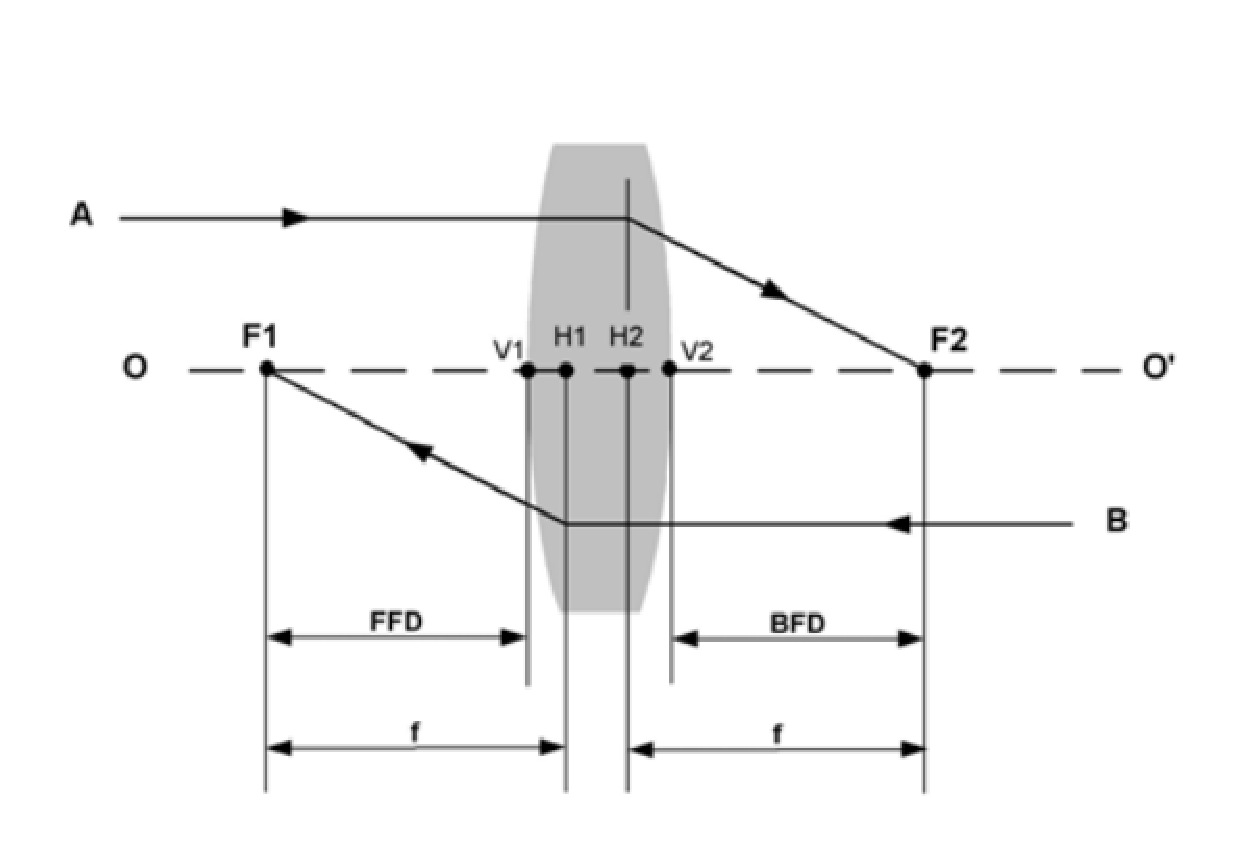
\includegraphics[width=0.33\textwidth]{bilder/lens_define}
\caption{The quantities define of singlet lenses}
\label{fig:lens_define}
\end{figure}

\begin{table}
\begin{tabular}{|c|c|c|}
\hline
Plano Convex & \parbox[c]{2.1cm}{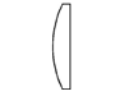
\includegraphics[width=2cm]{bilder/plano_convex}}& $f=\frac{R}{(n-1)}$ \\
\hline
Plano Concave &\parbox[c]{2.1cm}{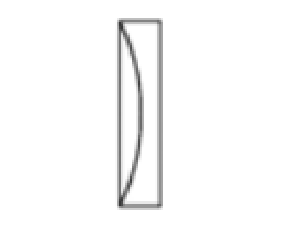
\includegraphics[width=2cm]{bilder/plano_concave}} & $f=-\frac{R}{(n-1)}$ \\
\hline
Equiconvex & \parbox[c]{2.1cm}{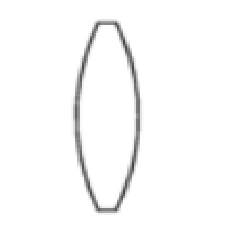
\includegraphics[width=2cm]{bilder/equi_convex}} & $f=[\frac{2(n-1)}{R} - \frac{t_{c}(n-1)^2}{nR^2}]^{-1}$ \\
\hline
Equiconcave & \parbox[c]{2.1cm}{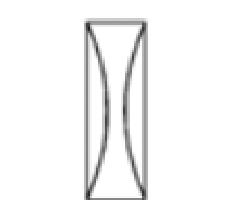
\includegraphics[width=2cm]{bilder/equi_concave}} & $f=[\frac{2(n-1)}{R} + \frac{t_{c}(n-1)^2}{nR^2}]^{-1}$ \\
\hline
\end{tabular}
\caption{Focal length Formulas of Simple Singlet Lenses in Air.  
				 The Radii are considered positive in the formulas below.}
\label{lenses_focal_length}
\end{table}



	